%%% Frontiers in Cognition --- Hypothesis & Theory
%%% Converted from paper/frontiers-smn-paper.md. Body budget <= 12,000 words
%%% (Frontiers counts main body + footnotes + in-text citations only).
%%% NB: logo1.eps must be in the path to compile the front-page header.

\documentclass[utf8]{FrontiersinHarvard} % Harvard (author-date); correct for Frontiers in Cognition

\usepackage{url,hyperref,lineno,microtype,subcaption}
\usepackage[onehalfspacing]{setspace}
\usepackage{amsmath,amssymb}
\usepackage{graphicx}
\graphicspath{{../../figures/}}

\linenumbers

\def\keyFont{\fontsize{8}{11}\helveticabold }
\def\firstAuthorLast{Nagarjuna {and} Karnam}
\def\Authors{G. Nagarjuna\,$^{1,*}$ and Durgaprasad Karnam\,$^{2}$}
\def\Address{$^{1}$Indian Institute of Science Education and Research (IISER) Pune, Pune, India \\
$^{2}$Indian Institute of Technology (IIT) Bombay, Mumbai, India }
\def\corrAuthor{G. Nagarjuna}
\def\corrEmail{nagarjuna@iiserpune.ac.in}

\begin{document}
\onecolumn
\firstpage{1}

\title[Haltability as the ground for object-directed cognition]{Haltability as the architectural ground for object-directed cognition: a falsifiable account, tested in silico}

\author[\firstAuthorLast ]{\Authors}
\address{}
\correspondance{}
\extraAuth{}

\maketitle

\begin{abstract}
\section{}
Cognitive science still lacks a single account that explains both the grounded, embodied character of animal cognition and the generative, symbolic character of human thought, and that does so in a way that can be put at risk. We advance such an account --- the \emph{Sensation Modulating Network (SMN)} --- and make a claim about \emph{what the nervous system does for cognition} that breaks with both received camps: against cognitivism, the nervous system is not a processor computing over representations; against 4E, it is not merely one strand of a brain--body--world loop. It is, first and most basically, an \emph{antagonistic modulator} --- an opponent network organized to oppose the ambient fields a body lives in (gravity, the medium) and to hold dynamic equilibria --- and cognition is what this organization produces when its dual interface turns on the sensory stream its own action generates. We then do two things the architecture's first statement did not. First, we sharpen the account into \emph{differential predictions} against the frameworks it is most often confused with (active inference, sensorimotor enactivism, equilibrium-point control), so observation can decide between them rather than accommodate each. The organizing claim is that \emph{haltability} --- the architectural capacity to actively hold a configuration still against an antagonistic balance, at a real metabolic cost we call \emph{alert energy} --- is the locus of object-directedness: an object is first registered as \emph{other} when it halts an ongoing action. Second, we test the architecture \emph{in silico} on an open, reproducible bench (SMN-Lab) built on a derived minimal model organism, with matched non-modulatory controls and pre-registered hypotheses. Across nine pre-registered studies the architecture is confirmed about as often as it is corrected: the world model is body-relative but does \emph{not} scale with raw transducer count; perceptual resolution scales with coordinated-zone density \emph{only} under active modulation; reafference separates self from world; and the reproduced signatures of haltability and antagonistic control hold. We argue that this confirm-and-correct ledger is itself the point: it distinguishes a mechanistic, falsifiable architecture from a principle that absorbs every mechanism. We state plainly what a simulation can and cannot carry --- structural signatures of object-directedness, not its phenomenology --- and identify the wet-lab measurement (the metabolic correlate of alert energy) that would decide the framework's strongest claim.

\tiny
\keyFont{ \section{Keywords:} embodied cognition, enactivism, reafference, haltability, opponent control, morphological computation, active inference, falsifiability}
\end{abstract}

\section{Introduction}\label{sec:intro}

Two research traditions divide the science of mind. \emph{Cognitivism} explains the generativity of thought --- its recursive, compositional, symbol-like productivity --- but floats free of the body that thinks. \emph{4E cognition} (embodied, embedded, enactive, extended) returns thought to the body and its world, but has been weaker on where recursive generativity comes from and, more damagingly for a science, weaker on \emph{falsifiable mechanism}. Neither tradition has produced a unified account that explains both the grounded character of animal cognition and the generative character of human thought --- and that can be wrong.

Underneath that division lies a deeper disagreement that the two camps rarely state outright: what is the nervous system \emph{for}? Answer that one question differently and everything downstream --- what perception is, where representation lives, what an experiment should measure --- changes with it. This paper's first contribution (Section~\ref{sec:camps}) is to answer it differently from both camps. Cognitivism's answer is that the nervous system \emph{computes} --- it builds and manipulates representations, and the body is peripheral input and output. 4E's answer is that the nervous system is \emph{one strand of a coupled loop} --- cognition is enacted across brain, body, and world. The \emph{Sensation Modulating Network (SMN)} gives a third answer: the nervous system is, first and most basically, an \emph{antagonistic modulator} --- an opponent network whose primitive job is to \emph{oppose} the ambient fields a body lives in and to \emph{hold} dynamic equilibria, and out of which cognition is constructed by modulating the sensation that action itself generates.

That is a claim about mechanism, and a mechanism can be wrong. So the rest of the paper does the two things the architecture's first statement \citep{NagarjunaKarnam2026SMN} did not.

\textbf{First, we sharpen the account against its rivals (Section~\ref{sec:falsify}).} A recurring and fair criticism of embodied-cognition frameworks is that they present a \emph{coherent alternative} without \emph{displacing} anything: they are consistent with the data and also consistent with their competitors. A theory earns its keep only where it predicts \emph{otherwise}. We therefore lay the SMN beside the three frameworks it is most often confused with --- active inference / the free-energy principle, \emph{sensorimotor enactivism}, and \emph{equilibrium-point control} --- and for each identify (i) what they share, (ii) where the SMN predicts differently, and (iii) the observation that would discriminate them. A shorter note treats Global Workspace Theory.

\textbf{Second, we test it in silico (Section~\ref{sec:ledger}).} Architectural claims about embodied cognition are usually \emph{illustrated} by a bespoke simulation, rarely \emph{risked} by one. We built SMN-Lab --- an open, reproducible bench on the MuJoCo physics engine, organized around a single \emph{derived} model organism --- specifically to risk the SMN: matched non-modulatory controls isolate which part of the body's organization did the work, pre-registered hypotheses fix pass/fail before running, seeded ensembles replace the single illustrative trial. The result is a \emph{confirm-and-correct ledger}, not a highlight reel.

The thesis tying everything together concerns \emph{haltability}. Classical accounts of action emphasize initiation; the SMN emphasizes the \emph{active hold}. A body built from opponent pairs can do what a body of independent effectors cannot: recruit a \emph{co-active equilibrium} in which two pulls cancel and a configuration is held still --- not by relaxing, not by inhibiting one side, but by spending energy to maintain a balance. We call the capacity \emph{haltability} and its state variable \emph{alert energy} ($E_R$), a non-negative, dimensionful quantity measuring the metabolic cost of the hold. Our central claim is that haltability is the \emph{architectural ground of object-directedness}. When an ongoing action meets a resistance it did not predict, the same antagonistic substrate that can hold a posture \emph{halts the action} --- and in that halt a portion of the world is registered, for the first time, as \emph{other than the self that was acting}. Aboutness does not require a symbol pointing at an object; it requires a body whose action can be stopped by what it is about. This is where the SMN parts company most cleanly from its neighbours, and where the bench has the most to say.

The paper proceeds: Section~\ref{sec:camps} makes the camp-level argument about what the nervous system does; Section~\ref{sec:arch} states the architecture; Section~\ref{sec:registers} lists the eight predicted registers as architectural fingerprints; Section~\ref{sec:falsify} is the comparative falsification; Section~\ref{sec:ledger} reports the in-silico results against those predictions; Section~\ref{sec:discussion} discusses what is confirmed, corrected, and open --- including what a simulation cannot carry and the single wet-lab measurement that would decide the framework's strongest claim; Section~\ref{sec:conclusion} concludes.

A note on what this paper is not. It is not a restatement of the preprint, and it does not claim to have \emph{measured} phenomenology. The bench tests the \emph{structural signatures} the SMN holds to constitute object-directedness; whether those signatures are \emph{sufficient} for experience or merely \emph{necessary} is the question the instrument is built to sharpen, not to settle (Section~\ref{sec:disc-sim}).

\section{What the nervous system does: the SMN against both camps}\label{sec:camps}

The longest-running disagreement in the cognitive sciences is usually fought over evidence, but its root is a prior commitment about the \emph{function} of the nervous system. Each camp has an implicit answer; the SMN's explicit answer is the wager of this paper. We state all three, keep what each camp gets right, and locate precisely where the SMN diverges --- because that divergence is what later sections turn into predictions and put at risk.

\subsection{Cognitivism: the nervous system computes}\label{sec:cog}

On the cognitivist picture, the nervous system is an information-processing organ. It builds representations of the world and manipulates them; cognition is computation over those representations; perception is the recovery of a world-model from input, and action is its output. The body is a transducer at one end and an effector at the other --- peripheral to the processing that \emph{is} cognition. The paradigm case is recursive generative grammar \citep{chomsky1957syntactic}: a biologically given, productive, compositional capacity that, on this view, has the form of symbol manipulation.

What cognitivism gets \emph{right} is substantial and we keep it: recursive generative capacity is real, it is phylogenetically given rather than relearned by each individual, and it is central to human cognition. A framework that cannot honour generativity has given up on what makes human thought distinctive. What cognitivism gets \emph{wrong} is the localization: it places that capacity in \emph{disembodied symbol-manipulation} and reduces the body to I/O. On this picture the antagonistic, motor organization of the nervous system is invisible --- muscles are output devices, not the substrate of cognition --- and the world-model is a god's-eye representation the agent recovers rather than a body-relative construction the agent makes.

\subsection{4E cognition: the nervous system as one strand of a loop}\label{sec:4e}

On the 4E picture --- embodied, embedded, enactive, extended --- cognition is not in the head. It is constituted by the dynamic coupling of brain, body, and environment; perception is something the agent \emph{does}, namely the mastery of sensorimotor contingencies; in its radical-enactivist forms, basic cognition is held to be representation-free.

What 4E gets \emph{right} we also keep: cognition is constitutively embodied, perception is action, and the body is not peripheral. But three things are left unsaid or got wrong, and a hypothesis-and-theory contribution must be candid about them. \emph{First}, the nervous system's specific \emph{architecture} is under-theorized. The strongest enactive statements --- Di Paolo, Buhrmann and Barandiaran's account of sensorimotor agency \citep{DiPaolo2017SensorimotorLife}, Thompson's developmental-systems enactivism \citep{Thompson2007MindInLife} --- are precise about the \emph{form} of the explanation (autonomy, sense-making, the brain--body--environment loop as a single dynamical system) but deliberately abstract about the \emph{parts}: ``the loop'' names the explanandum, and the nervous system tends to dissolve into one undifferentiated node within it, with little said about what makes it the node it is. The SMN's claim is that the node has a specific organization --- pull-only opponency, the dual interface, haltability --- and that this organization, not the loop-in-general, is what does the explaining. \emph{Second}, the radical-enactivist refusal of representation \citep{hutto2017} overshoots. An agent demonstrably acts on constructed, body-relative distinctions it is not currently sensing --- a foraging animal moves up a remembered gradient --- and a framework with no place for \emph{any} internal estimate cannot account for this. The SMN keeps a minimal, \emph{constructed} world model (a body-relative estimate maintained between coupled zones), which is neither the cognitivist's god's-eye representation nor radical enactivism's nothing. \emph{Third}, and most damaging for a science, much 4E work \emph{reframes} rather than \emph{predicts}: it is consistent with the data and with its rivals at once --- the very deficit this paper is built to remedy.

\subsection{The SMN's wager: cognition as antagonistic modulation}\label{sec:wager}

The SMN's answer is that the primitive operation of the nervous system is \emph{neither} computation over representations \emph{nor} a featureless dynamical coupling, but \emph{antagonistic modulation}. The nervous system is, at bottom, an opponent network whose first job is to \emph{oppose} the ambient fields the body cannot leave --- gravity, the medium --- and to \emph{hold} dynamic equilibria against them. Posture, before anything else, is the work of opposing the field; and cognition is what this opposing, holding organization produces when its \emph{dual interface} --- each element senses the very variable it moves --- turns on the sensory stream that its own action generates. This is a definite architecture (the opponent network of Coordinated Action Zones, Section~\ref{sec:arch}) with definite operations: \emph{opposition} (holding a balance against the field), \emph{modulation} (every act reshapes the sensation the acting element reads), \emph{reafference} (subtracting the self-caused part of that change), and \emph{haltability} (recruiting, at a real metabolic cost, a held state at which an unpredicted resistance registers as \emph{other}).

The move that distinguishes this from both camps is an \emph{inversion}. On the SMN account, distinctions are not \emph{read off} the world by transducers; they are \emph{constructed} by modulation. Self versus world is not detected by a dedicated sensor; it is the structural residual of acting while predicting. An object is not classified against stored categories; it is \emph{encountered} as what halts an action. Resolution is not a function of how many transducers fire but of how densely the body is coordinated and how actively it modulates --- the \emph{resolution principle}, which (tellingly) the bench both predicts and partly corrects (Section~\ref{sec:ledger}). Construction precedes structure: the nervous system \emph{makes} distinctions rather than \emph{finding} them already in the input.

This is a genuine third position, not a diplomatic relabeling, because it preserves each camp's truth by a \emph{substantive mechanistic commitment} that generates \emph{different predictions}:

\begin{itemize}
\item \textbf{With cognitivism, against its disembodiment.} Recursive generativity is real and biologically given --- but it is relocated from disembodied symbols to the modulable, recombinable dynamics of Negotiable Action Patterns on the opponent substrate. Generativity is \emph{grounded}, not free-floating; its externalized traces (gesture, vocalization, mark) are how it crosses body boundaries and becomes shareable.
\item \textbf{With 4E, against its mechanism-deficit and its anti-representationalism.} Cognition is constitutively embodied --- but the SMN supplies the nervous-system \emph{mechanism} (opponent zones, reafference, haltability) that 4E theorizing has sought without specifying, and it declines radical enactivism's elimination of representation: it keeps a \emph{body-relative world model} --- a constructed estimate anchored to opponent dynamics, neither a god's-eye picture nor nothing at all.
\item \textbf{Against both, the commitment neither makes.} A held state with a \emph{real metabolic price} --- alert energy --- whose dynamics are the shared substrate of attention \emph{and} the self/world distinction \emph{and} object-directedness. This is the commitment that makes the position falsifiable rather than merely reconciliatory: it predicts a measurable energetic signature (Section~\ref{sec:fep}, Section~\ref{sec:eph}) and a specific developmental order (self/world before object-directedness before symbolic generativity), and it is what Section~\ref{sec:ledger} puts at risk on the bench.
\end{itemize}

The stakes are simple to state. If the SMN is right, the explanatory centre of cognition is neither the representation (cognitivism) nor the coupling (4E) but the \emph{opponent loop} --- the antagonistic, field-opposing, sensation-modulating organization the nervous system is built from. (The same wager reframes a contemporary debate: it predicts that the difference between natural and artificial intelligence is not biology versus silicon but a \emph{dynamically constructed} opponent substrate versus a \emph{frozen training-time snapshot} whose context-perturbation dynamics simulate the surface of body-anchored cognition without its substrate --- a corollary we note here and develop elsewhere.) The remainder of this paper makes the wager predict otherwise than its neighbours, and then tries to break it.

\subsection{A developmental order, not a flat reconciliation}\label{sec:order}

A reconciliation that merely says ``keep the good parts of each camp'' is cheap and untestable. The SMN's reconciliation is different because it is \emph{ordered}: the architecture predicts a definite sequence in which the capacities each camp prizes become available --- each resting on the one before, none skippable --- and the order falls out of the morphology rather than being stipulated.

A single rigid body has mass and is subject to the field but generates no reafference: it can be displaced but cannot act --- a pure object. Add one joint (two segments) and the body can cause a sensory change \emph{and} predict it: the reafferent residual appears, and with it the first \emph{self/world} distinction --- though with a single reciprocating degree of freedom the body, by Purcell's scallop theorem \citep{Purcell1977LowRe}, goes nowhere. Add a second joint (three segments) and a non-reciprocal cycle becomes possible: the body can now carry its sensors \emph{through} the world, and the halt-at-resistance can single out a portion of that world, yielding \emph{object-directedness}. Only once an agent has object-directedness \emph{and} a layer of negotiable, recombinable action patterns does the recursive, externalizable generativity the cognitivist prizes --- \emph{symbolic} cognition --- become architecturally possible (Figure~\ref{fig:ladder}).

\begin{figure}[h!]
\centering
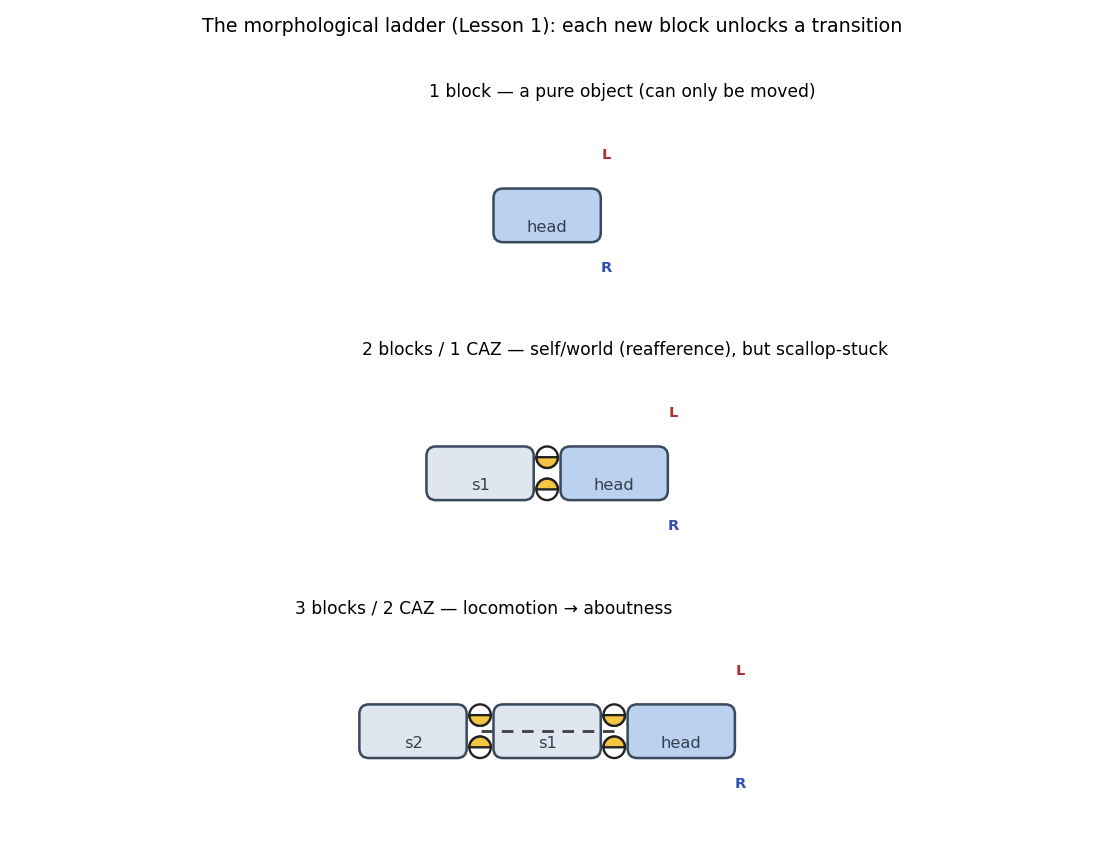
\includegraphics[width=0.62\linewidth]{morphology_ladder.png}
\caption{The morphological ladder. Each added block unlocks a transition. One block is a pure object (only displaceable). Two blocks (one CAZ) generate reafference and the self/world distinction but cannot locomote --- a single reciprocating degree of freedom is scallop-stuck. Three blocks (two CAZs) admit a non-reciprocal cycle, hence locomotion and the possibility of object-directedness. The split-circle glyph is a CAZ (opponent pair); L/R mark the bilateral axis.}
\label{fig:ladder}
\end{figure}

This staging is the substance of the reconciliation, not a gloss on it. 4E's embodiment claim is \emph{where the order starts}: self/world is \emph{built} from the opponent loop, not assumed. Cognitivism's generativity is \emph{where it ends}: recursion is real, but it is a late achievement grounded in the modulable action-pattern layer, not a primitive of mind. And the order is itself a source of risk. It predicts that self/world discrimination is present in bodies far too simple to have mastered any sensorimotor contingency or to manipulate symbols, and that \emph{no} amount of added representational machinery yields object-directedness in a body that cannot halt. Both are claims a bench --- or a comparative-developmental study --- can contradict. The minimal-organism derivation behind this ladder is exactly what fixes the bench's body plan (Section~\ref{sec:instrument}).

\section{The SMN architecture}\label{sec:arch}

The SMN is specified by a small set of commitments. We state the five the rest of the paper uses; the full six-commitment axiomatization and its formalism are in the preprint \citep{NagarjunaKarnam2026SMN}.

\subsection{Opponency at every scale}
The architecture's first commitment is that the elementary unit of biological control is not an effector but an \emph{opponent pair} --- two pull-only elements whose forces act against each other along a shared variable. Muscles come in antagonist pairs; so, the SMN argues, do control relations at every scale, from the flexor/extensor spanning a joint to the sympathetic/parasympathetic organization of autonomic tone. Opponency is not an implementation detail. A single pull-only actuator can only contract; a pair can hold, release, shift, and --- crucially --- \emph{stop}. The opponent pair is the smallest structure that has a stable \emph{held} state to depart from and return to.

\subsection{The Coordinated Action Zone}
The repeated unit is the \emph{Coordinated Action Zone (CAZ)}: an antagonistic, pull-only opponent pair spanning a joint, in which \emph{each end both senses and acts}. This is the \emph{dual interface} --- the CAZ is not a sensor wired to a motor but a single element that measures the very variable it moves. Sensing and acting are two readings of one coupling, not two modules joined by a wire. This is the architectural form of \emph{modulation of sensation through action}: every act changes the sensory surface the same element reads.

Two further commitments make the CAZ more than a servo. The agent is placed in a gravitational field treated as a structural prior --- an ambient, directional ordering the body did not choose and cannot leave --- and the CAZ's antagonism is organized to \emph{oppose} that field and the forces of the medium. The opponent pair holds a \emph{dynamic equilibrium}: a balance of physical forces, not a setpoint in a model. Posture, before anything else, is the work of opposing gravity; action is a \emph{departure from a balance}, not a command issued into a void. This locates the agent's elementary act in mechanics. And control is \emph{morphological computation} \citep{PfeiferBongard2006}: a network of CAZs coupled along the body performs work a central controller would otherwise do. The body is not a plant driven by a brain; in the relevant respect it \emph{is} the computer.

\subsection{The messaging beam}
CAZs are coupled by a \emph{messaging beam} --- nearest-neighbour phase coupling formalized as a Kuramoto-type chain \citep{Kuramoto1984Oscillations},
\begin{equation}
\dot\theta_i = \omega_i + \sum_{j\in\mathcal N(i)} K_{ij}\sin(\theta_j - \theta_i - \varphi_{ij}) + u_i,
\label{eq:kuramoto}
\end{equation}
where $\theta_i$ is the phase of zone $i$, $K_{ij}$ the coupling, $\varphi_{ij}$ a phase lag, and $u_i$ a sensory bias. From local coupling alone a coherent traveling wave emerges with no centre; a bilateral sensory gradient biases the wave into directed movement. The beam is also where the network's \emph{shared state} lives: the world model is not stored in any one segment but \emph{between} the segments, in the coupled state the beam maintains. By the same token the world model is constructed in the agent's own body geometry --- a body-relative frame, not a god's-eye coordinate system. What an agent can differentiate about its world is a property of how its zones are placed and coupled, not of a transducer count. (This last claim is one the bench tests directly, and partly corrects; Section~\ref{sec:ledger}.)

\subsection{The transducer and the reafference principle}
A \emph{transducer} registers that something is happening at a sensory surface; it cannot, by itself, tell whether the happening was caused by the agent or by the world. The SMN resolves this with the \emph{reafference principle} \citep{vonHolstMittelstaedt1950,CrapseSommer2008}: each CAZ carries a \emph{reafference predictor} that, from its own motor state, predicts the sensory change its action should produce, and subtracts it. The \emph{residual} --- observed minus predicted --- is small when a change is self-generated (the predictor tracks) and large when it is world-generated (the prediction is outdated). This residual is the architecture's primitive signal of \emph{self versus world}, and it generalizes: the SMN distinguishes self-contact, world-contact, and contact-with-another-agent as three structurally different residual signatures (the \emph{dual-signal property}, DS-1--DS-4; Section~\ref{sec:registers}, Registers 5 and 8).

When the predictor's world-model term is allowed to adapt (learning rate $\kappa>0$), the residual following a world change \emph{decays} --- and the rate of that decay is exactly mastery of a sensorimotor contingency in O'Regan and No\"e's sense \citep{OReganNoe2001Sensorimotor}, now rendered measurable rather than stipulated (Register 4).

\subsection{Haltability and alert energy}\label{sec:haltability}
Here is the architecture's distinctive move. \emph{Haltability} is the capacity to actively hold a configuration still --- distinct from passive relaxation and from classical inhibition. It is a property of the antagonism between the two zones, \emph{not} something the controller generates. Two pull-only zones whose forces oppose along a shared variable \emph{admit} a co-active equilibrium in which the forces cancel and the configuration is held without motion. This state is not produced; it \emph{exists} because the structural coupling makes it exist --- as the gravitational coupling of a constrained mass makes a pendulum's stable attractor exist. The controller does not generate the held state; it \emph{recruits} the affordance: reads the afferents, supplies activations that put both zones into co-activation, and maintains that against perturbation.

The state variable of this recruitment is the \emph{alert energy} $E_R$: a non-negative scalar measuring the metabolic cost of maintaining the co-activation. Its dynamics are simple: $E_R$ accumulates while a zone is actively driven, in proportion to the load it carries; it decays passively when not driven; when a halt is released, load-driven build-up resumes. Maintaining co-activation against the body's antagonistic affordance is \emph{real metabolic work} --- the recruitment is expensive even though the affordance it recruits is structural.

Three consequences matter for what follows. (1) \emph{Alert energy is treated as a real metabolic quantity}, not a free parameter: it is bounded, dimensionful, and decays passively, and the architecture predicts it should be measurable as the metabolic difference between an engaged-but-not-active zone and the same zone at rest. (2) \emph{Active equilibrium is a special case}: under load, $E_R$ grows until build matches decay, and the steady state is exactly the load-scaled co-activation. (3) \emph{The distinction from classical inhibition is sharp}: classical inhibition has no alert energy --- the inactive zone is at baseline or silenced, with no recruited affordance to maintain. The dynamics of $E_R$ are precisely what the SMN claims biological tissue does and reciprocal inhibition does not.

From halt to \emph{directedness}. With a surprise term active, an unpredicted sensory event during ongoing action drives the residual above an auto-halt threshold that gates the active drive within one integration step (Register 6). The \emph{same} alert-energy substrate that distinguishes haltability from inhibition is therefore also the substrate of \emph{attention}: a surprising affordance change disrupts cognitive inertia and stops the action. And in that stop, the resistance that caused it is registered as \emph{not-self} --- the architectural birth of object-directedness. This is the thesis the bench is built to probe and the rivals are arranged to contrast.

\subsection{Networks, layers, and what an implementation must commit to}
A single CAZ has a held state and a residual; a \emph{network} of CAZs has posture, gait, and a shared world model. The preprint treats the multi-CAZ network as a \emph{hybrid graph-dynamical system}: a graph whose nodes are CAZs and whose continuous dynamics are the phase-oscillator chain above, with a \emph{broadcast operator} ($\Pi$) that makes one zone's state available to another's predictor. Action patterns are organized in layers --- basal autonomic patterns (BAPs), habitual patterns (HAPs), and negotiable/self-modulatable patterns (NAPs/SMAPs) --- that recruit and modulate one another. The full analytical treatment of network stability, controllability, and convergence is, by the preprint's own statement, deferred. This deferral is exactly the gap SMN-Lab was built to fill empirically: a working multi-CAZ implementation in which the network-level claims can be \emph{exercised} even where they are not yet \emph{proved} (Section~\ref{sec:ledger}).

\section{The eight registers as architectural fingerprints}\label{sec:registers}

The architecture's value as science is that it commits to \emph{registers} --- concrete, measurable behavioural signatures, each derived from the formalism, each of which a real or simulated system either exhibits or does not. There are eight (seven testable, one explicitly hypothetical). We list them compactly; Section~\ref{sec:falsify} uses them as the discriminators against rival frameworks, and Section~\ref{sec:ledger} reports which the bench reproduces.

\begin{enumerate}
\item \textbf{Tonic load coupling.} During steady engagement of one zone, the partner's tonic activation rises \emph{linearly with the active zone's load}, $a_{\text{partner}}\approx a_0+\beta\rho\tau_E F_{\text{active}}$. Classical inhibition predicts $a_{\text{partner}}=a_0$, independent of load. \emph{(The clean discriminator against reciprocal inhibition.)}
\item \textbf{Resumption latency.} After a brief halt, the latency to reach a small reversed target is \emph{shorter} under SMN than under classical inhibition, by $\Delta t\approx \gamma E_R(t_{\text{release}})/K_p$ --- controlled by the alert energy still present at release.
\item \textbf{Reafference (self vs world).} For a fixed sensor change, the residual $|r|$ is small when self-generated, large when world-generated; in the noiseless limit the self-residual is identically zero. The \emph{Reafferenzprinzip} as a quantitative signature.
\item \textbf{Sensorimotor-contingency mastery.} With world-model adaptation on, the post-world-change residual decays to the noise floor; the decay \emph{is} mastery, measurable. O'Regan--No\"e rendered empirical.
\item \textbf{Intra-body dual-signal residual.} For two CAZs of one SMN sharing a sensory substrate, regressing the residual on the partner-as-stimulus form gives $R^2\to 1$; for a decoupled control reading an exogenous stimulus, $R^2\to 0$. A \emph{structural}, not magnitude, signature --- diagnostic, not confounded by noise level.
\item \textbf{Surprise-driven attention and auto-halt.} An unpredicted event drives the residual above threshold and gates the drive within one step; attention and haltability share one substrate.
\item \textbf{Shared intentionality (hypothesis).} Two agents in mutual reafference, both adapting, show a joint residual that decays far faster than under asymmetric or no adaptation ($\sim$92\% reduction in the reference simulation). Flagged as hypothesis \citep{Tomasello2005Understanding}.
\item \textbf{Self / world / other (dual-signal contrast).} A unifying re-presentation: the three Dual-Signal Indices ($\mathrm{DSI}^{\text{int}}$, $\mathrm{DSI}^{\text{ext}}$, $\mathrm{DSI}^{\text{cross}}$) give a three-way structural distinction between broadcast-internal contact, contact with a non-intentional exterior, and contact with another agent's structured modulation. The architecture makes the distinction \emph{available}; it does not claim the agent thereby \emph{has} a rich self/world/other.
\end{enumerate}

Three further network-level consequences (BAP-backdrop entrainment, axial$\leftrightarrow$appendicular mode-switching latency, Hebbian NAP recruitment) follow from the formalism but presuppose a multi-CAZ implementation; the preprint flags them as targets rather than numbering them. They are precisely what a bench can reach --- and Section~\ref{sec:ledger} reaches some of them.

The registers are the architecture's falsifiers. A framework that produced none of them, or whose competitors produced all of them equally, would be idle. The next section asks the second question --- \emph{do the competitors produce them?} --- and the section after that asks the first --- \emph{does the architecture, when built, actually exhibit them?}

\section{Comparative falsification: where the SMN predicts otherwise}\label{sec:falsify}

A theory of embodied cognition is only as strong as the bets it is willing to lose. The camp-level divergence of Section~\ref{sec:camps} becomes useful only when it yields \emph{differential predictions}. We place the SMN beside the three frameworks with which it shares the most, and for each give: \emph{shared ground}, the \emph{divergent prediction}, and the \emph{discriminating observation} --- flagging which observations SMN-Lab can adjudicate in silico and which require the wet lab.

\subsection{Active inference / the free-energy principle}\label{sec:fep}
\textbf{Shared ground.} Both frameworks make \emph{prediction error} central \citep{Friston2010FreeEnergyPrinciple,ParrPezzuloFriston2022}. The SMN's reafference residual is a prediction error; its surprise-driven auto-halt is, in the loosest sense, surprise minimization; its layered action patterns resemble a hierarchy. An active-inference theorist can re-describe almost every SMN mechanism as a special case of free-energy minimization, and this is exactly the difficulty.

\textbf{Where the SMN predicts otherwise.} The divergence is not about whether prediction error matters but about \emph{what does the holding}. In active inference, action is in the service of inference: the agent acts to make its sensations match its predictions, and ``resistance'' is a high prediction-error state to be explained away by updating beliefs or sampling differently. There is no privileged \emph{mechanical} quantity; the generative model is substrate-neutral all the way down. In the SMN, the hold is mechanical and metabolically costly before it is inferential: haltability is a structural affordance of an antagonistic pair, and alert energy $E_R$ is a \emph{real metabolic quantity with specific dynamics} --- it accumulates with load, decays over seconds, and is the cost of maintaining a co-active equilibrium. The SMN predicts a measurable energetic signature where active inference predicts, at most, a free-energy bookkeeping with no commitment to its physical realization.

\textbf{Discriminating observation.} Register 1 (tonic load coupling) and the haltability dynamics: the SMN predicts that the antagonist's tonic activation tracks agonist load \emph{linearly} and that, after release, this co-activation decays over seconds to tens of seconds rather than vanishing immediately --- and that this corresponds to a real metabolic cost (measurable, in principle, by combined EMG and NIRS / $^{31}$P-MRS in sustained isometric tasks). Active inference makes no such commitment; it is compatible with the signature being present \emph{or absent}. That asymmetry is the test: a framework compatible with both outcomes cannot claim the outcome as evidence. SMN-Lab adjudicates the in-silico half --- that an opponent pair \emph{recruited and held} at a metabolic cost yields antagonistic benefits scaling with load (Section~\ref{sec:preds}, Pred-3) --- while the biological metabolic correlate is the decisive wet-lab measurement the framework still owes (Section~\ref{sec:disc-measurement}).

\textbf{The falsifiability asymmetry.} There is a second, sharper contrast, methodological rather than empirical. The free-energy principle has been charged --- by sympathizers as well as critics --- with being effectively \emph{unfalsifiable}: a principle so general that it absorbs any mechanism as one of its special cases. The SMN takes the opposite stance by construction: it commits to eight registers with explicit functional forms, any of which a measurement can contradict --- and, as Section~\ref{sec:ledger} reports, \emph{three pre-registered SMN predictions were corrected by our own bench}. A framework that can be wrong, and was, is doing different epistemic work from a principle that cannot be. We do not claim this makes the SMN \emph{true}; we claim it makes the SMN \emph{testable} in a way its most powerful neighbour is not, and that this is the relevant virtue for a hypothesis-and-theory contribution.

\subsection{Sensorimotor enactivism}\label{sec:enact}
\textbf{Shared ground.} O'Regan and No\"e's sensorimotor enactivism \citep{OReganNoe2001Sensorimotor} holds that perception is constituted by the \emph{mastery of sensorimotor contingencies} --- the lawful ways sensory input changes as the agent moves. The SMN endorses this and, in Register 4, renders it measurable: mastery is the decay of the reafference residual under world-model adaptation. On this point the SMN is enactivism's friend, supplying a mechanism for a thesis usually stated at the level of competence.

\textbf{Where the SMN predicts otherwise.} Sensorimotor enactivism is, by design, silent on the \emph{wiring-level} mechanism that distinguishes self-caused from world-caused sensory change --- it locates the difference in \emph{mastery}, a global achievement of the agent. The SMN locates it in a \emph{local structural signature}: the dual-signal property (DS-1--DS-4) predicts that self-contact, world-contact, and other-contact produce \emph{structurally different residuals} (Registers 5, 8), distinguishable by the \emph{form} of the residual (the $R^2\to1$ vs $R^2\to0$ regression), not merely by an agent's downstream success. The SMN therefore predicts a self/world distinction that is available before, and independent of, mastery --- present in the residual geometry of a single CAZ pair, not only in a trained agent's skilled coping.

\textbf{Discriminating observation.} The structural residual signature: an agent that has \emph{not} mastered a contingency should still exhibit the dual-signal contrast (self-residual structurally distinct from world-residual) if the SMN is right, whereas a pure mastery account predicts the distinction emerges only with skilled engagement. \emph{SMN-Lab adjudicates this} (Sections~\ref{sec:s1}--\ref{sec:q1}): reafference separates self from world on the crawler, and --- the sharper, partly \emph{corrective} result --- the self/world resolution collapses as the body grows unless the modulation is active, which says the distinction is carried by the architecture's modulatory wiring, not by transducer count or accumulated mastery alone.

\subsection{Equilibrium-point / referent control}\label{sec:eph}
\textbf{Shared ground.} Feldman's equilibrium-point hypothesis and its referent-control successors \citep{Feldman1986_EquilibriumPoint,Feldman2015ReferentControl,Latash2008EquilibriumPointHistory} are the SMN's closest kin in motor control: movement is generated by shifting the equilibrium of antagonist muscle pairs, not by computing torques. The SMN's ``action is a departure from a balance'' is an equilibrium-point claim, and the SMN inherits the EPH's central insight that the opponent pair, not the single muscle, is the unit.

\textbf{Where the SMN predicts otherwise.} The EPH has no \emph{alert energy} and no \emph{haltability} as a distinct, costly, actively-maintained state. In the EPH, holding a posture is just commanding an equilibrium; there is no separate prediction that the \emph{cost} of the hold scales with load and decays over seconds, and no claim that this cost is the substrate of attention and object-directedness. The SMN adds exactly this: tonic load coupling that \emph{exceeds} what reciprocal-inhibition models predict (Register 1) and a post-release resumption advantage governed by residual alert energy (Register 2). Equilibrium-point and referent-control studies report co-activation broadly consistent with this picture but have \emph{not} tested the specific load-scaling and post-release-decay predictions --- which is precisely the open space the SMN occupies.

\textbf{Discriminating observation.} Registers 1 and 2: the load-linearity of antagonist tone and the seconds-scale decay after release, plus the resumption-latency advantage. SMN-Lab adjudicates the mechanical half (Section~\ref{sec:preds}): co-contraction produces antagonistic benefits --- faster perturbation correction --- that grow with perturbation size, at a roughly \emph{quadratic} energy cost, exhibiting the load-scaled tradeoff the SMN predicts and the bare EPH does not model. The biological load-scaling and decay constants remain the wet-lab discriminator.

\subsection{The resolution principle: against precision-weighting and receptor density}\label{sec:resolution}
\textbf{Shared ground.} Every account of perception must explain \emph{acuity} --- why an agent can make some discriminations and not others. Two standard answers bracket the SMN's. Classical psychophysics ties acuity to \emph{receptor density and sampling}: more transducers, finer grain. Predictive-processing accounts tie it to \emph{precision-weighting} --- the gain placed on prediction error according to a learned estimate of its reliability. Both make resolution something the agent \emph{has}, whether in its receptor sheet or in its precision parameters.

\textbf{Where the SMN predicts otherwise.} The SMN's \emph{resolution principle} makes acuity a property of \emph{active organization}: resolution is a function of coordinated-zone density \emph{times} active modulation, and --- the sharp, counter-intuitive part --- raw transducer count contributes \emph{nothing on its own}. Adding sensors to a body that does not modulate the sensation they deliver does not improve, and can even degrade, what the body can discriminate: unmodulated afferents add noise to a body-relative estimate rather than detail. Precision-weighting is the closer kin (it too denies that more input is automatically more information), but it locates the gain in an \emph{inferential parameter}, whereas the SMN locates it in a \emph{structural-dynamical} fact --- whether the body's zones are coupled and actively sampling. This is the inversion of Section~\ref{sec:wager} in its most testable form: acuity is \emph{constructed} by modulation, not \emph{possessed} by the sensor sheet.

\textbf{Discriminating observation.} Hold modulation off and vary transducer count: a receptor-density account predicts acuity rises; the SMN predicts it does not, and that self/world resolution can \emph{fall} as the sensor sheet grows. \emph{SMN-Lab adjudicates this directly} (Sections~\ref{sec:s1}--\ref{sec:q1}): added segments and sensors do not improve the world model (S1), and self/world resolution \emph{collapses} with body size unless modulation is active (Q1) --- while \emph{with} modulation, resolution rises with zone density (Q1b). This is the bench's cleanest differential result, and the one that most surprised us: it overturned our own pre-registered prediction (Section~\ref{sec:s1}), exactly the kind of bet a precision or receptor account is not structured to lose.

\subsection{Global Workspace Theory (a shorter note)}\label{sec:gwt}
Global Workspace Theory \citep{Baars2005GlobalWorkspace,Dehaene2014Consciousness} proposes that conscious access consists in broadcasting specialized content to a shared workspace. The SMN's broadcast operator $\Pi$ provides a \emph{structural} mechanism for such a shared state --- but the two are not competitors so much as accounts pitched at different levels. The SMN's contribution here is to ground ``broadcast'' in a concrete network operation (cross-zone availability of state to a partner's predictor) with measurable consequences (the dual-signal indices of Register 8), rather than in a metaphor of a workspace. We flag this as positioning, not falsification: the discriminating experiments would require a multi-CAZ implementation exercising $\Pi$ at scale, which the network-level consequences of Section~\ref{sec:registers} anticipate but the present bench only partially reaches.

\subsection{Summary}\label{sec:falsify-summary}
The pattern across Sections~\ref{sec:fep}--\ref{sec:resolution} is consistent. The SMN agrees with each rival on a shared core --- prediction error (active inference), sensorimotor mastery (enactivism), equilibrium shifting (EPH), the demand for an account of acuity (predictive processing) --- and then makes one \emph{additional, mechanical, costly} commitment the rival does not: \emph{a held state with a real metabolic price, whose dynamics are the substrate of attention, the self/world distinction, and a resolution that is constructed rather than possessed.} That commitment generates registers a rival is compatible-with-either-way, which is exactly what makes them discriminating. The remaining question is whether the architecture, when actually built, exhibits them. That is what the bench is for.

\section{Testing the architecture in silico: the SMN-Lab ledger}\label{sec:ledger}

\subsection{The instrument, briefly}\label{sec:instrument}
SMN-Lab is an open-source embodied simulation bench (MuJoCo; GPL-3.0; \url{https://github.com/gnowgi/smn-lab}) built to \emph{risk} the SMN rather than illustrate it. Five commitments make its results count as tests. (1) A \emph{derived model organism}: in an overdamped world, Purcell's scallop theorem \citep{Purcell1977LowRe} forbids net displacement to any body with a single reciprocating degree of freedom, so the smallest body that can \emph{initiate non-inertial movement} --- and therefore carry its sensors \emph{through} a world to ask directional questions of it --- is a \emph{three-segment axial chain} (two joints, a non-reciprocal cycle). Scaling is then a parameter, not a redesign, and the same primitives compose a whole body family (Figure~\ref{fig:menagerie}). (2) A \emph{dual-interface CAZ} as the unit: an antagonistic pull-only opponent pair that senses the joint it moves. (3) A strict \emph{engine boundary}: MuJoCo supplies rigid-body dynamics, contact, and actuation; the architecture supplies CAZs, the messaging beam, the action patterns, and the constructed world model; chemical and thermal fields the engine does not simulate are computed bench-side as virtual scalar fields sampled at sensor sites. (4) Pre-registration with matched non-modulatory foils: every experiment fixes hypothesis, order parameter, a control identical \emph{except for the one thing the SMN says matters}, and pass/fail, before running. (5) \emph{Seeded, self-describing datasets}: a sweep harness runs each experiment across a parameter grid and a seed ensemble and stamps the exact code commit, so results are reproducible and the ``small-data'' objection dissolves.

\begin{figure}[h!]
\centering
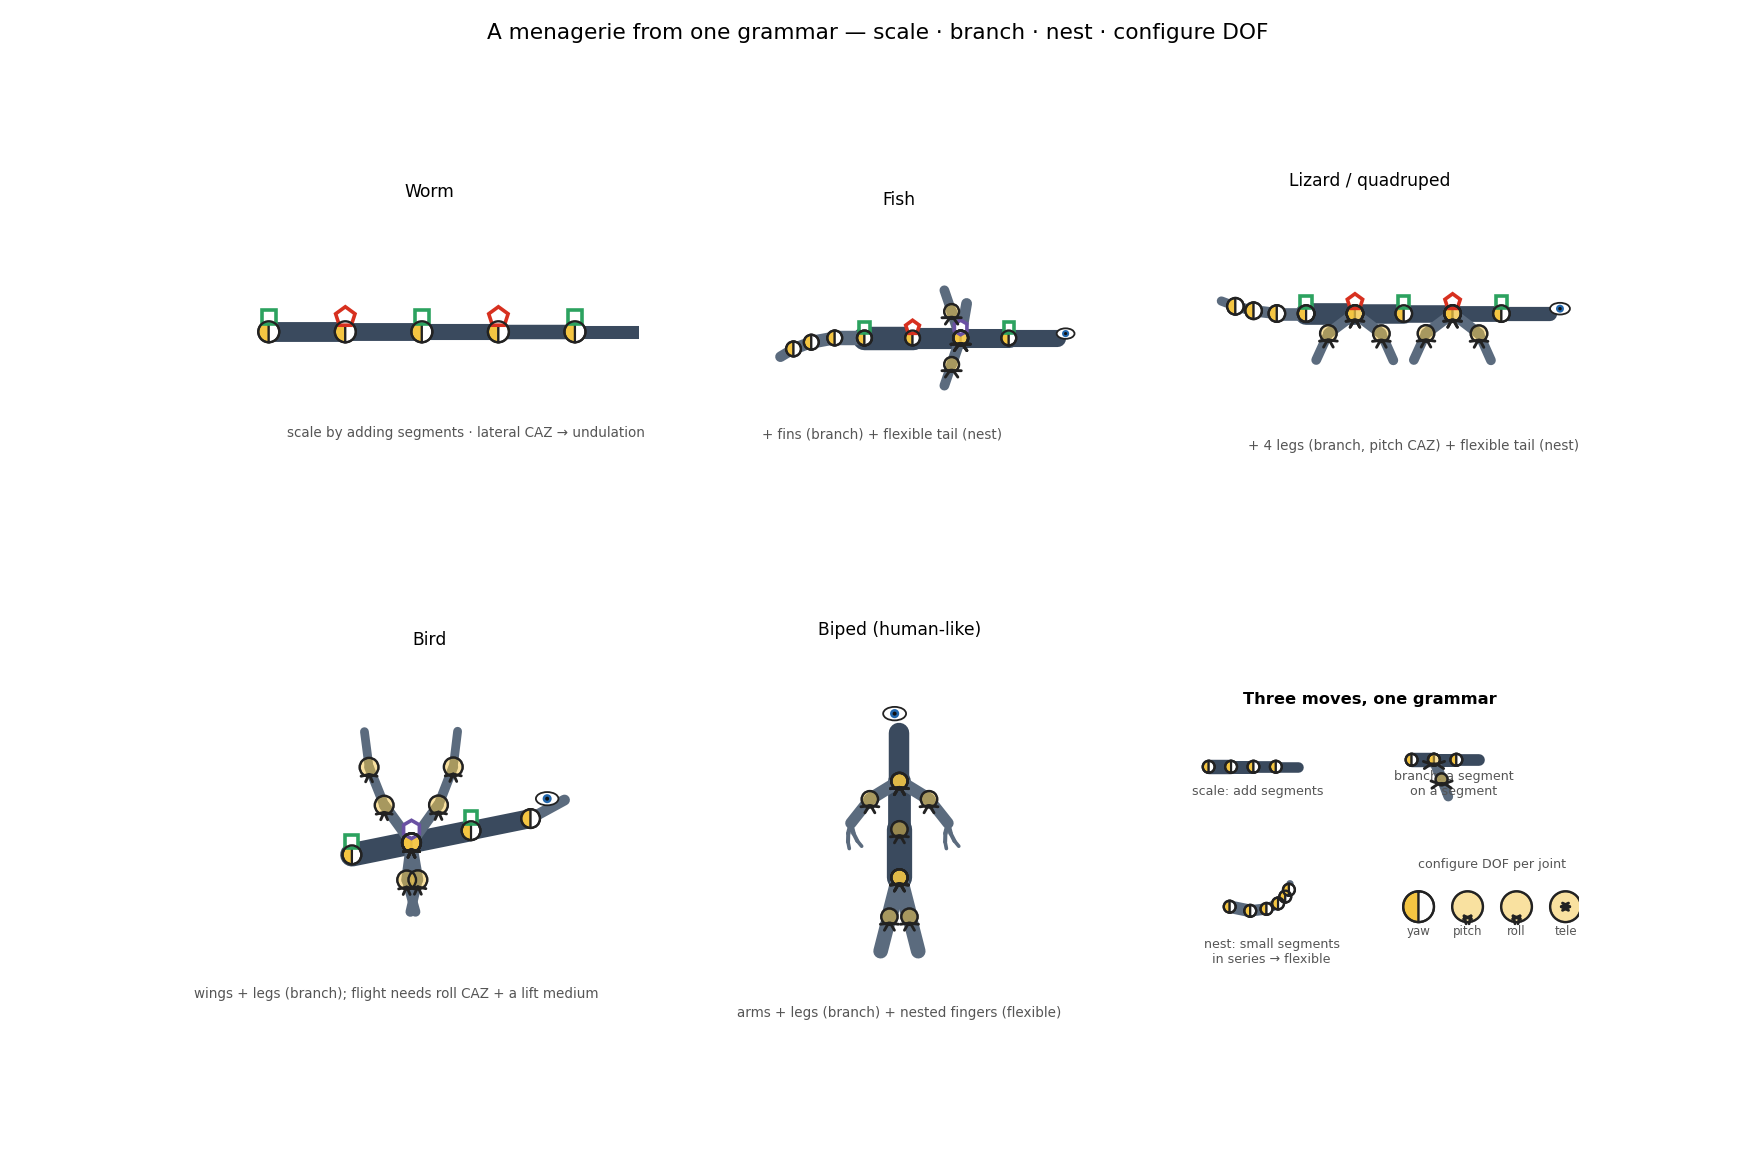
\includegraphics[width=\linewidth]{menagerie.png}
\caption{A menagerie from one grammar. Worm, fish, lizard/quadruped, bird, and biped are built from the same primitives by four moves: \emph{scale} (add segments), \emph{branch} (a chain attached to a segment --- a leg, wing, or antenna), \emph{nest} (small segments in series make a flexible part --- a tail or finger), and \emph{configure} each joint's CAZ degree of freedom (yaw, pitch, roll, telescoping). Complexity is composed, not redesigned, so the unit of analysis --- segment, CAZ, sensor, coupling --- stays fixed across the family.}
\label{fig:menagerie}
\end{figure}

A discipline of integrity governs reporting: adjustments forced during an experiment --- and especially anything beyond the published architecture --- are \emph{declared explicitly}; confounded runs are \emph{discarded, not reported}; and a pre-registered prediction that fails is recorded as a \emph{correction}, not quietly dropped. What follows is the ledger that discipline produced.

\subsection{Locomotion is a network effect (S0, confirmed)}\label{sec:s0}
\emph{Prediction.} If the messaging beam's coupling is what organizes locomotion, then a coupled chain should produce coherent directed travel while a matched chain with coupling set to zero should not.

\emph{Result.} The matched non-modulatory foil (coupling $=0$) travels $0.56\pm0.28$ m --- occasionally far by chance, with huge variance --- while the coupled chain travels $0.75\pm0.002$ m, with variance collapsing roughly \emph{100-fold}. The diagnostic is not the mean distance (a flailing body sometimes drifts far) but the \emph{collapse of variance}: coupling converts undirected thrashing into a reproducible gait. This is morphological computation made measurable, and it is the template for the whole C-series --- a matched foil isolating the one structural variable (Figure~\ref{fig:s0}). \emph{Confirmed.}

\begin{figure}[h!]
\centering
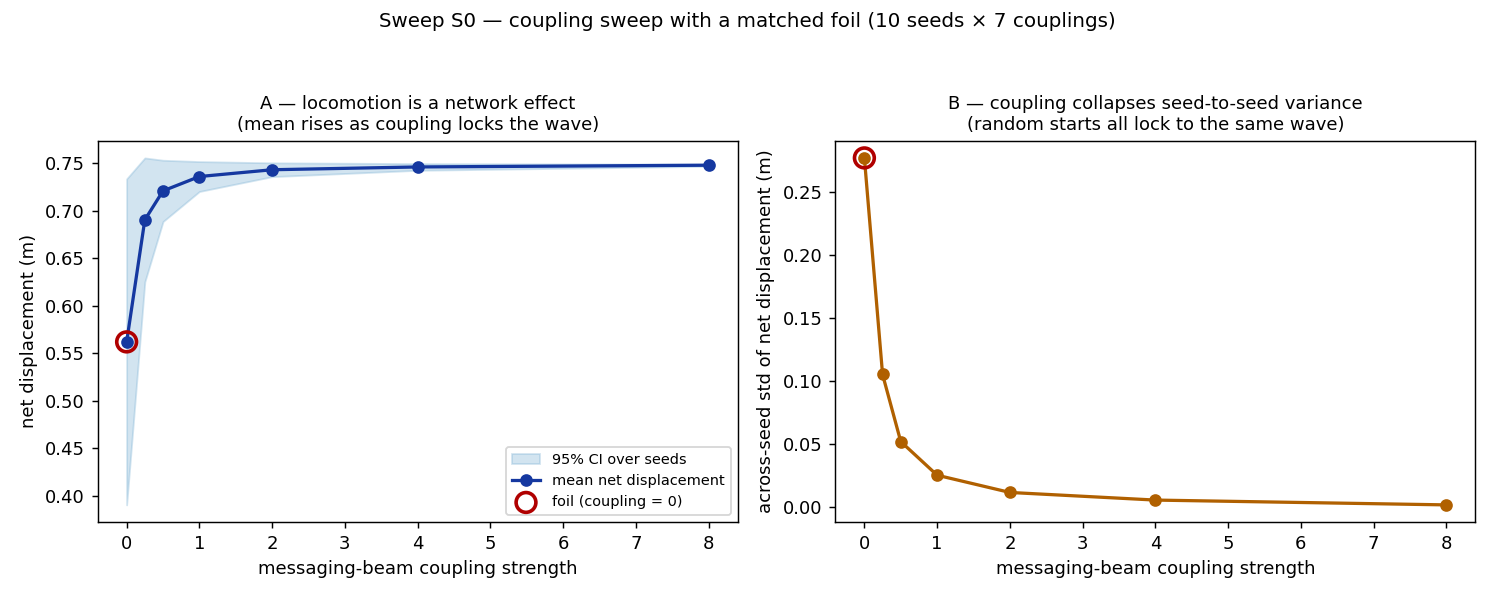
\includegraphics[width=\linewidth]{sweep_c0_coupling.png}
\caption{S0 --- locomotion is a network effect (10 seeds $\times$ 7 couplings). (A) Net displacement rises as messaging-beam coupling locks the traveling wave. (B) The diagnostic is variance: across-seed standard deviation collapses roughly 100-fold as coupling increases, as random starts all lock to the same gait. The matched foil (coupling $=0$, red ring) flails --- occasionally far, but unreproducible.}
\label{fig:s0}
\end{figure}

\subsection{The world model is body-relative --- but does not scale with raw geometry (S1, corrected)}\label{sec:s1}
\emph{Pre-registered prediction.} A body-relative world model exists, \emph{and its fidelity rises with segment count} (more sensors, more coverage $\to$ a better world model).

\emph{Result.} A held-out $k$-nearest-neighbour decoder recovers the agent's position from its internal state well above a shuffled baseline (skill $\approx 0.4$ vs $\approx 0$) at \emph{every} body size --- confirming a real body-relative world model (Register 4 territory). But the fidelity is \emph{flat in segment count}: more segments, more sensors, and more coverage do \emph{not} improve it. Our pre-registered ``rises with $n_{\text{seg}}$'' was \emph{wrong}, and we record it as a correction.

\emph{Why it matters.} The null is consistent with the SMN's own \emph{resolution principle}: raw transducer count adds no resolution by itself. This is the first place the bench corrected the framework's na\"ive reading and redirected the live question from \emph{geometry} to \emph{modulation} --- setting up Section~\ref{sec:q1}. (The first run of this study was confounded by large-body instability and collapsed exploration; it was discarded, and the clean re-run used declared adjustments --- anterior-only steering, longer run.)

\subsection{Resolution scales with zone density only under modulation (Q1, Q1b)}\label{sec:q1}
This is the pivotal pair, and it splits into a corrected sub-claim and a confirmed one.

\emph{Q1 (modulation, core claim confirmed; one sub-claim corrected).} With per-zone dual-interface modulators (each zone predicting its \emph{own} motion), modulation cancels self-caused sensory change to the noise floor at \emph{all} body sizes. Crucially, \emph{without} modulation the self/world resolution \emph{collapses} as the body grows: the foil's world-detection ratio falls from $13.7$ to $1.2$ as segments go $3\to9$, while the modulation advantage \emph{widens} with density ($8.5\times \to 22\times$). Raw transducer count without modulation \emph{subtracts} resolution. (The pre-registered sub-claim that the \emph{modulated absolute} ratio rises with $n_{\text{seg}}$ was wrong --- a localized stimulus dilutes the whole-body mean; recorded as a correction, and the narrow claim left open for Q1b.)

\emph{Q1b (resolution, confirmed).} With a \emph{distributed} stimulus (a uniform global ``tide,'' removing the localized-dilution confound), the modulated world-detection ratio \emph{rises with density} ($14 \to 22.6$, scaling roughly as $1/\sqrt N$) while the foil falls ($2.5 \to 1.4$). Perceptual resolution scales with CAZ density --- \emph{but only with modulation}. This is the first C-series prediction \emph{confirmed without correction}, and the bench's cleanest vindication of the resolution principle: density helps \emph{if and only if} the body actively modulates (Figure~\ref{fig:q1b}).

\begin{figure}[h!]
\centering
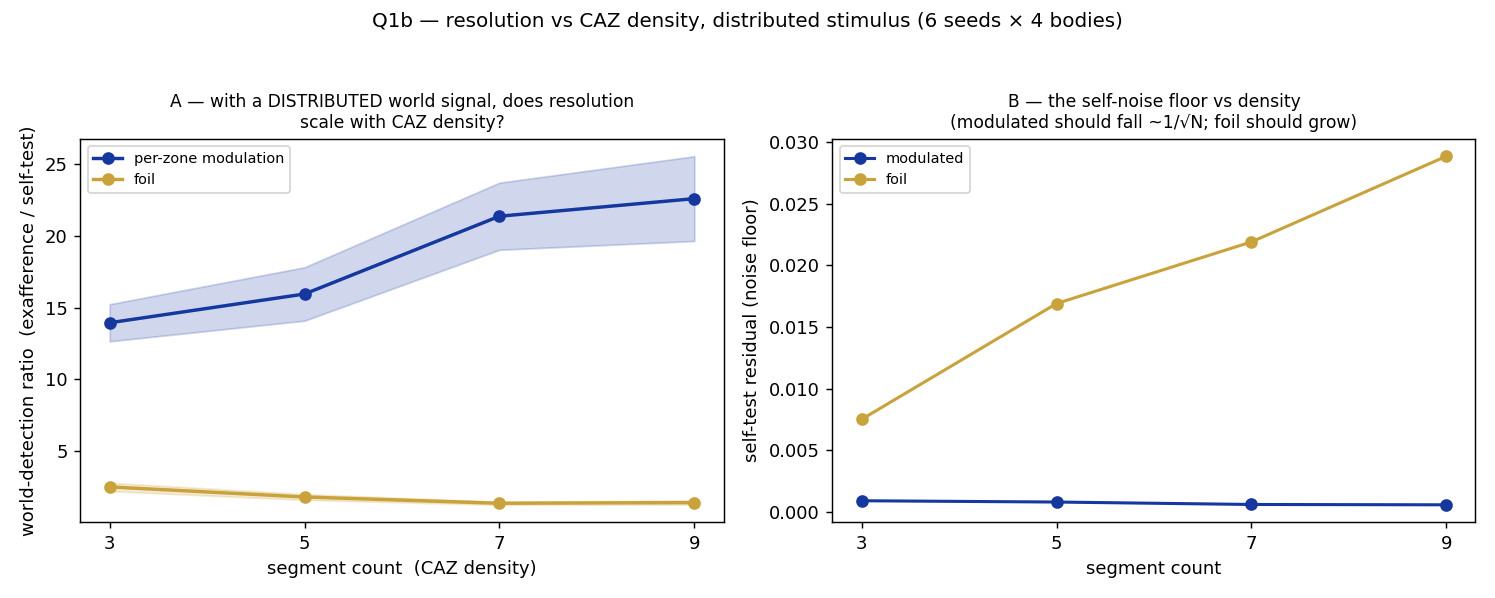
\includegraphics[width=\linewidth]{sweep_q1b_resolution.png}
\caption{Q1b --- resolution scales with CAZ density, but only under modulation (6 seeds $\times$ 4 bodies, distributed stimulus). (A) The per-zone-modulated world-detection ratio rises with segment count ($\sim$14 $\to$ 22.6) while the matched non-modulatory foil falls. (B) The self-noise floor: the modulated residual stays near zero (falling $\sim 1/\sqrt N$) while the foil's grows with body size. Density helps if and only if the body actively modulates.}
\label{fig:q1b}
\end{figure}

\emph{Bearing on Section~\ref{sec:falsify}.} This pair is the discriminating result against sensorimotor enactivism (Section~\ref{sec:enact}): the self/world distinction is carried by the modulatory wiring, not by transducer count or accumulated mastery --- exactly the SMN's wiring-level prediction, and the in-silico face of the inversion argued in Section~\ref{sec:wager}.

\subsection{Reafference separates self from world (Q2, partial)}\label{sec:q2}
\emph{Prediction (Register 3).} The reafference predictor cancels self-caused sensory change, leaving world-caused change intact --- a residual ratio favouring world over self.

\emph{Result.} On the crawler, reafference cancels $\sim$\emph{37\%} of self-caused change, giving a self/world ratio of \emph{2.2} versus a matched foil's \emph{1.58} --- supported, but \emph{not} the clean Register-3 result obtained in the preprint's single-CAZ reference simulation. The honest reason is structural: a single head-velocity proprioceptive signal cannot predict \emph{distributed} sensors on a \emph{bending} body, so cancellation is incomplete. We report this as \emph{partial}, and flag a methodological scar candidly: across modeling choices the measured ratio swung between 1.3 and 5.5, and we settled on the principled regime (a linear field with a moving source, where the predictor's model is \emph{exact}) rather than the choice that flattered the result. This is the integrity discipline doing its job.

\subsection{Three reproduced architectural predictions}\label{sec:preds}
The preprint itself calls for ``quantitative predictions through computational modelling.'' We reproduced three.

\emph{Pred-1, haltability signatures (confirmed).} In a deceptive-reach task, a \emph{haltable} controller imposes a distinct stop --- velocity to zero with a dwell of $\sim$\emph{0.17 s} plus a discrete opponent-pair \emph{re-pairing} --- where a smooth foil shows none. The dwell, not the zero-crossing, is the diagnostic (a direction reversal forces \emph{any} controller through zero). Importantly, the halt is a signature, not a speed gain: the haltable agent reacquires the target \emph{later}, by exactly the dwell. This matters for Section~\ref{sec:falsify}: haltability is a real, detectable mechanical event, not a re-description of slowing down --- the in-silico realization of Register 6 (Figure~\ref{fig:pred1}).

\begin{figure}[h!]
\centering
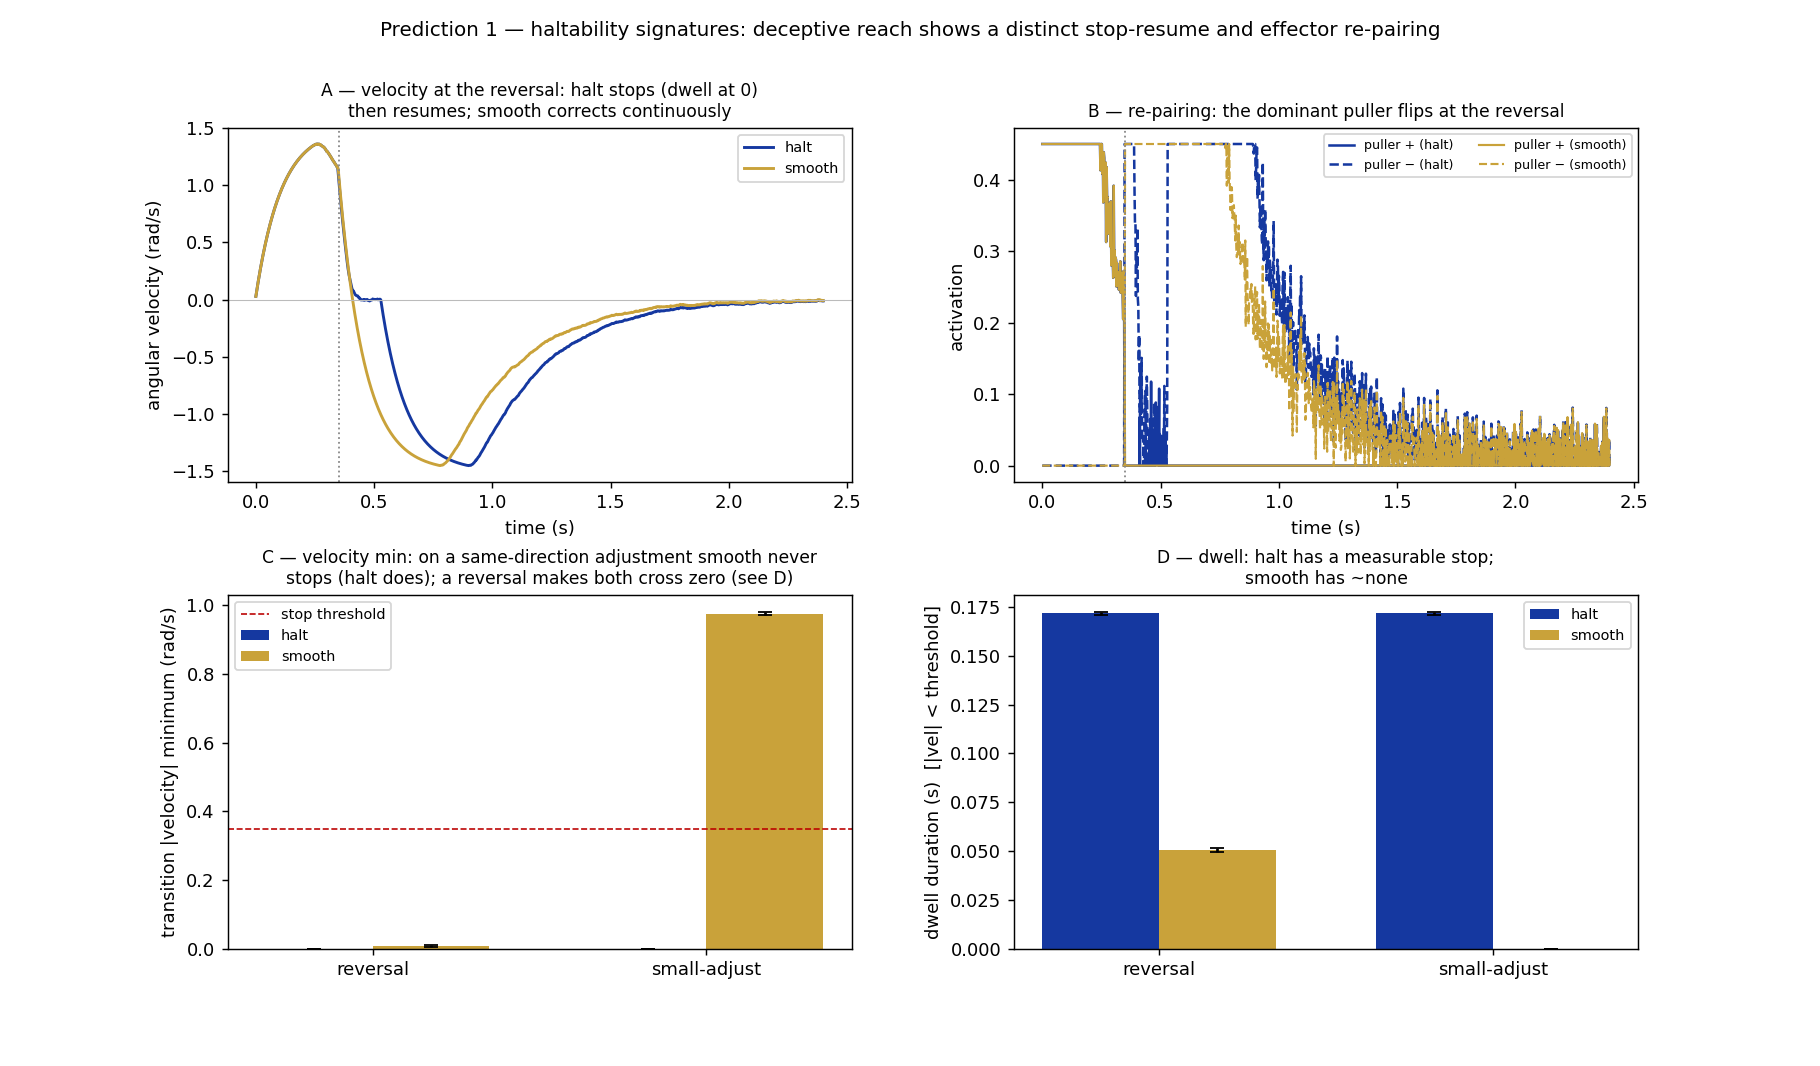
\includegraphics[width=0.95\linewidth]{sweep_pred1_haltability.png}
\caption{Pred-1 --- haltability signatures in a deceptive reach. (A) At the reversal the haltable controller stops (angular velocity to zero) then resumes, where the smooth foil corrects continuously. (B) Re-pairing: the dominant opponent (puller) flips at the reversal. (C) On a same-direction adjustment the smooth foil never crosses zero, so (D) the diagnostic is the \emph{dwell} --- a measurable stop ($\sim$0.17 s) --- not the zero-crossing; the smooth foil shows none.}
\label{fig:pred1}
\end{figure}

\emph{Pred-2, zonal dissociations (partial).} The optimal control gain moves with the substrate, and a compliant tool punishes aggressive control catastrophically (a 60$\times$ spread in error across gains). But a conservative \emph{generic} prior performs about as well as substrate-specific tuning on \emph{both} substrates, so the strong reading --- that the architecture \emph{needs} substrate-specific priors --- is \emph{not} supported: the dissociation is one catastrophic corner, not a true two-way crossover. Recorded as \emph{partial}, with the strong claim explicitly \emph{not} claimed.

\emph{Pred-3, antagonistic benefits (confirmed).} Co-contraction speeds perturbation correction (peak deviation $-4.4\times$, integrated absolute error $-28\times$), with the benefit \emph{larger for larger perturbations}, at a roughly \emph{quadratic energy cost} --- the load-scaled tradeoff of Section~\ref{sec:eph}. This required a \emph{declared adjustment}: the original force-motor co-contraction was inert for stiffness (opposed force-motors simply cancel), so we added a muscle-impedance plus neural-delay model, and we state that this goes beyond the preprint's actuator. With it, the opponent pair held at a metabolic cost yields exactly the antagonistic benefit the SMN predicts and the bare EPH does not model --- the in-silico half of the Section~\ref{sec:fep} and Section~\ref{sec:eph} discriminators.

\subsection{The ledger}\label{sec:ledger-table}
\begin{table}[h!]
\centering
\begin{tabular}{p{3.2cm} p{5.2cm} p{5.2cm}}
\hline
\emph{Study} & \emph{SMN prediction} & \emph{Outcome} \\
\hline
S0 coupling & locomotion is a network effect & \emph{confirmed} (variance collapses $\sim$100$\times$) \\
S1 geometry$\to$world-model & body-relative model, \emph{scales with geometry} & model \emph{confirmed}, scaling \emph{corrected} (flat) \\
Q1 modulation & modulation carries self/world resolution & core \emph{confirmed}; one sub-claim \emph{corrected} \\
Q1b resolution & resolution scales with zone density (with modulation) & \emph{confirmed} ($1/\sqrt N$) \\
Q2 reafference & self/world separation by reafference & \emph{partial} (37\% cancellation; distributed-body limit) \\
Pred-1 haltability & distinct active halt signature & \emph{confirmed} (dwell $\sim$0.17 s) \\
Pred-2 zonal & substrate-specific priors required & \emph{partial} (strong reading not supported) \\
Pred-3 antagonism & antagonistic benefit at load-scaled cost & \emph{confirmed} ($-28\times$ IAE, $\sim$quadratic cost) \\
\hline
\end{tabular}
\caption{The confirm-and-correct ledger across nine pre-registered studies. Plus three confounded runs caught and discarded before reporting.}
\label{tab:ledger}
\end{table}

The arithmetic of Table~\ref{tab:ledger} is the argument: across nine pre-registered studies the architecture was confirmed about as often as it was corrected. An instrument that only ever confirmed its theory would be an illustration; this one is a test. That is the empirical answer to the falsifiability asymmetry of Section~\ref{sec:fep} --- the SMN is the framework that can be wrong, and here it is, on the record, being wrong in specific, informative ways.

\section{Discussion}\label{sec:discussion}

\subsection{What the ledger buys the theory}\label{sec:disc-ledger}
The corrections are worth more to the theory than the confirmations. The two that bite --- the world model does \emph{not} improve with raw geometry (Section~\ref{sec:s1}), and self/world resolution \emph{collapses} without modulation (Section~\ref{sec:q1}) --- converge on a single sharpened claim: \emph{the SMN's explanatory work is done by modulation, not by transduction.} More sensors, more segments, more coverage buy nothing on their own; they buy resolution only when the body actively modulates the sensation they deliver. This is the resolution principle promoted from a stated commitment to a measured result, and it is exactly the inversion of Section~\ref{sec:wager} made quantitative: distinctions are constructed, not read off. Had we only run the confirmations, we would have a weaker theory and not known it.

\subsection{Addressing the architecture's known gaps}\label{sec:disc-gaps}
An independent novelty assessment of the SMN preprint named four weaknesses; the bench speaks directly to two and clarifies a third. The charge that the multi-CAZ network analysis was deferred is met in kind: S0, Q1/Q1b, and Pred-1--3 are multi-CAZ demonstrations exercising coupling, density, and opponent dynamics in a working network, even where the closed-form stability theory remains open. The charge of \emph{limited substrate independence} --- that the preprint's reference simulations all used a Hill-type muscle model --- is partly met by construction: SMN-Lab's actuators are simple \emph{pull-only opponent motors}, not Hill-type, so the registers it reproduces are already shown in a \emph{different} physical realization; Pred-2 further varies the substrate (rigid vs viscoelastic). The charge that the SMN does not attempt falsification against established findings is reframed rather than met: the bench falsifies \emph{against the architecture's own pre-registered predictions} (and corrected three), which is falsification in practice; comparative falsification against established frameworks is Section~\ref{sec:falsify}'s differential predictions plus the wet-lab measurement of Section~\ref{sec:disc-measurement}.

\subsection{What a simulation can and cannot carry}\label{sec:disc-sim}
We state the irony plainly rather than finesse it: SMN-Lab offers an \emph{embodied} agent inside a \emph{simulation}. A simulation is not a body and has no phenomenology; nothing here is claimed to feel anything. What MuJoCo \emph{does} provide is \emph{real physics} --- gravity, contact, drag, opponent forces --- and what the bench instantiates is the \emph{structural and relational} conditions the SMN holds to constitute object-directedness: a body-relative frame, the reafferent separation of self from world, the dual interface that measures while it moves, and the halt at resistance through which an object announces itself as \emph{other}. These are exactly what a physics simulation can carry, and they are what our experiments measure. The felt, first-person character of experience is neither captured nor claimed. The bench therefore tests the \emph{signatures} of object-directedness, not its phenomenology. Whether those signatures are \emph{sufficient} for experience, or merely \emph{necessary}, is the question the instrument is built to sharpen, not to settle --- and stating that boundary precisely is, we think, worth more than papering over the irony.

\subsection{The decisive measurement the framework still owes}\label{sec:disc-measurement}
The SMN's strongest and riskiest claim is that alert energy is a real metabolic quantity, not a model parameter --- that maintaining a co-active antagonistic hold costs energy that accumulates with load and decays over seconds. The bench can show the \emph{functional consequences} of such a quantity (Pred-3: antagonistic benefit at a load-scaled cost), but it cannot measure biological metabolism. The clean test is in the wet lab: combined EMG and metabolic measurement (NIRS, $^{31}$P-MRS) during sustained isometric tasks, looking for antagonist tonic activation that tracks agonist load \emph{linearly} (Register 1) and decays over \emph{seconds to tens of seconds} after release rather than vanishing immediately. A positive result would distinguish the SMN sharply from both classical reciprocal inhibition and the bare equilibrium-point hypothesis; a null would falsify the framework's central energetic commitment. We name this as the experiment that matters most, and as one we cannot run on the bench --- an honest boundary of the in-silico method.

\subsection{Limitations and roadmap}\label{sec:disc-limits}
The present studies use planar idealizations and a single organism family (the axial crawler and its menagerie of scaled/branched/nested variants). The network-level consequences of Section~\ref{sec:registers} --- BAP-backdrop entrainment, axial$\leftrightarrow$appendicular mode-switching latency (an HKB-style phase transition \citep{HakenKelsoBunz1985}), Hebbian NAP recruitment --- are anticipated but only partly reached, and the broadcast operator $\Pi$ awaits an experiment at scale. Two mechanism gaps remain \emph{declared, not filled}: haltability-to-object \emph{selection} (Q3) and cross-modal binding (Q4). The natural next moves are a multi-CAZ network study targeting $\Pi$ and mode-switching, the social extension to \emph{perceptual crossing} \citep{Auvray2009PerceptualCrossing,FroeseDiPaolo2010PerceptualCrossing} (object-directedness $\to$ other-directedness, probing Register 7 and the boundary of Section~\ref{sec:disc-sim}), and reproductions of recognized minimal-cognition paradigms (Beer's categorical perception \citep{Beer2003}; Braitenberg vehicles; the Enactive Torch's sensory-substitution paradigm \citep{EstelleFroese2025EnactiveTorch} hosted in a synthetic agent) --- each adding the bench's distinctive move: a matched foil that says \emph{which part of the body's organization did the work}. The bench already ships a Brooks-style subsumption controller as a foil \citep{Brooks1991}.

\section{Conclusion}\label{sec:conclusion}

We set out to answer one question the two camps leave implicit --- \emph{what does the nervous system do for cognition?} --- and then to make our answer earn its keep. The answer is that the nervous system is an \emph{antagonistic modulator}: an opponent network that opposes the fields a body lives in, holds dynamic equilibria, and constructs distinctions by modulating the sensation its own action generates. Neither cognitivism's computing organ nor 4E's featureless loop, it keeps what each camp got right --- generativity, embodiment --- while supplying the mechanism each lacks, and adds the commitment neither makes: a held state with a real metabolic price.

The unifying claim is that \emph{haltability} --- that active, costly hold --- is the architectural ground of object-directedness: an object is first registered as \emph{other} in the moment an unpredicted resistance halts an ongoing action. From this one commitment the SMN diverges from active inference (which has no privileged mechanical, costly hold), from sensorimotor enactivism (which locates the self/world distinction in mastery rather than in a local structural signature), and from the equilibrium-point hypothesis (which shifts equilibria but does not price the hold) --- and the divergences take the form of registers a measurement can contradict.

Built and tested, the architecture was confirmed about as often as it was corrected. Locomotion is a genuine network effect; resolution scales with coordinated-zone density, but \emph{only} under active modulation; the world model is body-relative but does \emph{not} improve with raw geometry; reafference separates self from world; and the signatures of haltability and antagonistic control reproduce. The corrections matter most: they show the explanatory work lies in modulation, not transduction, and they show an instrument doing what frameworks of embodied cognition too rarely permit --- putting the theory at risk and recording where it fails. The single measurement the framework still owes --- the metabolic correlate of alert energy --- is the experiment we most want done, and the one the bench cannot do. A theory worth this much says clearly what would refute it. This is ours, and here is where it has already been wrong.

\section*{Conflict of Interest Statement}
The authors declare that the research was conducted in the absence of any commercial or financial relationships that could be construed as a potential conflict of interest.

\section*{Author Contributions}
GN and DK jointly developed the SMN architecture and its theoretical argument, over a sustained collaboration of about ten years carried out alongside their professional commitments as science-education researchers. The biological and philosophical grounding, and the recognition of the need to seek an alternative framework, originated with GN. SMN-Lab was developed by GN with AI-assisted code. Both authors read and approved the submitted manuscript.

\section*{Funding}
% TODO: add funding sources / grant numbers, or state none.

\section*{Data Availability Statement}
All code, documentation, and seeded datasets for SMN-Lab are openly available at \url{https://github.com/gnowgi/smn-lab} (GPL-3.0); documentation at \url{https://smn-lab.readthedocs.io}.

\bibliographystyle{Frontiers-Harvard}
\bibliography{references}

\end{document}
